%%%%%%%%%%%%%%%%%%%%%%%%%%%%%%%%%%%%%%%%%%%%%%%%%%%%%%%%%%%%%%%%%%%%%%%%%%%%%%%
%% 2.- DESARROLLO DEL PROYECTO
%%%%%%%%%%%%%%%%%%%%%%%%%%%%%%%%%%%%%%%%%%%%%%%%%%%%%%%%%%%%%%%%%%%%%%%%%%%%%%%

\cleardoublepage
\chapter{Desarrollo del proyecto}
\chaptermark{Desarrollo del proyecto}

\label{chap:desarrolloProyecto} % etiqueta para poder referenciar luego en el texto con ~\ref{sec:intro}
% \addcontentsline{toc}{chapter}{Introducción, Objetivos, Metodología y Planificación

En las siguientes secciones se detalla de forma estructurada el desarrollo de cada una de las partes que componen este proyecto.


\section{Programación iPro}
\label{sec:programacionipro}
Como ya se ha explicado en los capítulos anteriores, el destino del iPro es la programación de la UTA existente en el supermercado. En el \hyperref[chap:anexoUTA]{Anexo~\ref{chap:anexoUTA}} se describe detalladamente qué es una UTA y todos los elementos de los que se puede componer. Para el caso que nos atañe, la \hyperref[tab:especificacionesUTA]{Tabla~\ref{tab:especificacionesUTA}} recoge las especificaciones concretas del control.

\begin{table}[H]
    %\centering
    \begin{center}
      \setlength\arrayrulewidth{2pt}
      \resizebox{0.8\linewidth}{!}{\begin{tabular}{ | c | c c c c | }
        %\Cline{2pt}{2-5}
        \hhline{|*{5}{-}}
        \cellcolor{lightgray}\textbf{GRUPO} & \multicolumn{1}{c|}{\cellcolor{lightgray}\textbf{Entrada analógica}} & \multicolumn{1}{c|}{\cellcolor{lightgray}\textbf{Salida analógica}} & \multicolumn{1}{c|}{\cellcolor{lightgray}\textbf{Entrada digital}} & \cellcolor{lightgray}\textbf{Salida digital}   \\ \hline
        \footnotesize{\textbf{Ventiladores}} &  & \parbox[c][1.6cm]{0.2\linewidth}{\centering\footnotesize{Ventilador impulsión\\Ventilador retorno}}  & \parbox[c][2.6cm]{0.2\linewidth}{\centering\footnotesize{Seguridad Ventilador impulsión\\Seguridad Ventilador retorno}} &  \\ \hline
        \footnotesize{\textbf{Filtros}} & & & \footnotesize{\parbox[c][2cm]{0.2\linewidth}{\centering{Filtro entrada\\Filtro salida\\Filtro retorno}}} & \\ \hline
        \footnotesize{\textbf{Humectador}} & \footnotesize{\parbox[c][1.2cm]{0.2\linewidth}{\centering{Humedad de retorno\\Humedad exterior}}} & & \centering\footnotesize{Indicador nivel agua} & \footnotesize{ON/OFF Humectador} \\ \hline
        \footnotesize{\textbf{Intercambiador de calor}} & \footnotesize{\parbox[c][1.2cm]{0.2\linewidth}{\centering{Temp. impulsión agua\\Temp. retorno agua}}} & & & \footnotesize{Válvula de agua}\\ \hline
        \footnotesize{\textbf{E/S de aire}} & \footnotesize{\parbox[c][2.7cm]{0.2\linewidth}{\centering{Temp. impulsión aire\\Temp. retorno aire\\Temp. extracción aire\\Temp. aire exterior}}} & & & \\ \hline

      \end{tabular}}
      \caption{Especificaciones E/S UTA.}
      \label{tab:especificacionesUTA}
    \end{center}
  \end{table}

La lógica de funcionamiento se recoge en el diagrama de flujo de la Figura xxx, y sigue las siguientes pautas:

\begin{itemize}
  \item \textbf{Compuertas:} No existen compuertas regulables.
  \item \textbf{Filtros:} La señal digital de los filtros indica si están sucios o no.
  \item \textbf{Ventiladores:} 
  \begin{itemize}
    \item La velocidad de los ventiladores se regula mediante una señal 0-10V, dicha velocidad debe ser la misma en cada momento.
    \item La señal digital en los ventiladores indica fallo en los mismos.
    \item La velocidad debe ser regulable de forma automática o de forma manual:
    \begin{itemize}
      \item La regulación automática ajusta la velocidad del ventilador en función de la diferencia de temperatura con la consigna.
      \item La regulación manual de la velocidad se establece en tres rangos parametrizables: alta, media y baja.
    \end{itemize}
  \end{itemize} 
  \item \textbf{Humectador:} 
  \begin{itemize}
    \item Se establece una consigna de humedad.
    \item A partir de las mediciones de humedad del aire que entra y sale se activa la humectación o no.
    \item El indicador de nivel del humectador indica si éste está lleno o no.
  \end{itemize}
  \item \textbf{Intercambiador de calor:}
  \begin{itemize}
    \item Debe existir un aviso que indique si el fluido está a una temperatura acorde para alcanzar la consigna deseada.
    \item Mientras la UTA esté en funcionamiento, la válvula que lleva el fluido hasta el intercambiador debe estar abierta.
  \end{itemize}
  \item \textbf{E/S de aire:}
  \begin{itemize}
    \item La temperatura de retorno es la usada como referencia para el control de temperatura del aire.
    \item El control de temperatura se establece según el modo de funcionamiento: verano (frío) o invierno (calor).
    \item Las curva de funcionamiento para cada uno de los modos es la de la \hyperref[figura:curvasModos]{Figura~\ref{figura:curvasModos}}:
  \end{itemize}
\end{itemize}

\begin{figure}[H]
  \centering
  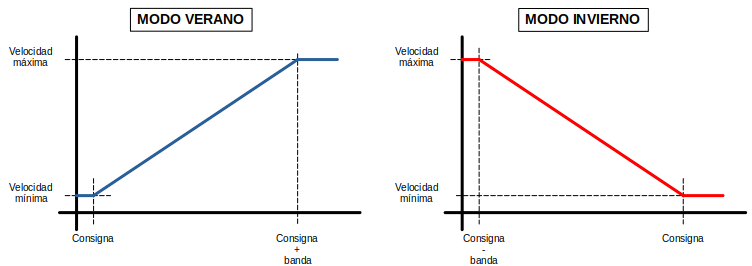
\includegraphics[width=\textwidth, keepaspectratio]{img/curvaModos}
  \caption{Modos de funcionamiento}
  \label{figura:curvasModos}
\end{figure}


\section{Diseño Pantalla para el control}
\label{sec:programacionpantalla}
indican las conclusiones generales obtenidas a partir del estudio realizado, se proponen lineas de trabajo futuro, y se indican las publicaciones asociadas al trabajo realizado en este TFM.
\section{Elaboración de librerías en Kiconex}
\label{sec:librerias}
indican las conclusiones generales obtenidas a partir del estudio realizado, se proponen lineas de trabajo futuro, y se indican las publicaciones asociadas al trabajo realizado en este TFM.
\section{Programación dispositivo wireless}
\label{sec:programacionesp32}
indican las conclusiones generales obtenidas a partir del estudio realizado, se proponen lineas de trabajo futuro, y se indican las publicaciones asociadas al trabajo realizado en este TFM.